For $z\lesssim 2$, large fractions of predicted baryon contents are missing in observations.  
The majority of them are believed to reside in warm-hot intergalactic mediums (WHIM) with typical temperature of $10^5$ K to $10^7$ K \cite{Pen1999,Soltan06}. 
High temperature and low density in the medium, 
as well as uncertainties in ionization states and metalicities, 
make it difficult to derive information from metal absroption lines. 
It is expected urgently for probes that not only trace the majority of the baryons, but also can be interpreted model-independently.

Among proposed probes, the kinematic Sunyaev-Zel'dovich (kSZ) effect \cite{Sunyaev72,Sunyaev80,Vishniac87} is a promising one.  
kSZ effect results from Compton scattering of cosmic microwave background (CMB) off free electrons. 
The radial velocity of electrons will give photon a Doppler shift 
and hence leads to a 
secondary anisotropy in CMB temperature.
%The kSZ signal could satisfy all three conditions listed before. 
%Consider kSZ as tracer has lots of advantages for this problem. 
It is an ideal probe to tackle the problem: 
First, it contributes from all the free electrons, indicating the distribution of $90\%$ of the baryons in ionized states,   
leaving alone only less than $10\%$ of baryons that 
reside in stars, remnants, atomic and molecular gases \cite{Fukugita04}. 
%
Second, the signal is mainly influenced by electron density and radial velocity, 
regardless the temperature, pressure and metalicity,  
so no extra assumptions are needed to estimate baryon abundance.  
%
Third, the peculiar velocity is dominantly related to large scale structures, 
therefore the signal is less biased towards local mass contractions, 
and more indicative about diffusive distributions.  

Attractive as it is, two drawbacks largely reduce the feasibility of harnessing kSZ signal.  
First, the signal is weak 
and hence suffers seriously from contaminations 
from primary CMB, facility noises, 
thermal SZ effect, CMB lensing, etc.  
Second, it is an integrated effect along line of sight, therefore, kSZ itself does not contain redshift information.

A straight-forward mitigation of the disadvantages is to cross correlate 
kSZ signal with another tracer, which has both large scale structure and redshift information. 
Previous work has proposed optical spectroscopic survey as an ideal tool \cite{Hand12,Shao11,Li14}. 
%However, lack of spectral lines in redshift $1.4-2.5$, and low survey speed has limited the application.  
However, lack of prominent spectral lines at redshift $1.4-2.5$ 
makes it difficult to consistently measure evolution from $z>2$ to $z=0$. 
%And kSZ signal is more prominent at $z\sim2$ than $z<1.4$, 
%making it painful to leave out this stretch.
Moreover, the high requirements on facilities and sources 
largely constraint the sky coverage it could reach, 
especially when redshift goes up, 
which limits it to relatively small angular scales, 
with very low level of primary CMB. 
%
Methods trying to relax requirements on density fields, such as 
cross correlating photo-z galaxies with kSZ \cite{Hill16,Ferraro16}, 
depend on models of velocity fields and   
demand next generation CMB facilities, eg. 
ACTpol, CMB-S4 
to achieve 
convincing S/N.

%Optical spectroscopic surveys have been proposed as an ideal candidate. 
%Opitical spectroscopic surveys are one popular candidate. 
%However, they are not accessible on redshift $1.4-2.5$ 
%when all the lines are shifted away. 
%To consistently measure the sky from $z=0$ to $z=2$, we consider harness the H~I $21$ cm  line in radio band, which can also provide accurate redshift information.
%Rather than distinguishing individual galaxies, 
%we discuss the possibility of using integrated signals of each pixel 
%(intensity mapping) 

In this paper, a new possibility of cross correlating HI density field from 21 cm intensity mapping(IM) to kSZ signal is discussed. 
HI 21 cm spectra have accurate redshift information, 
and are fully accessible for $z\lesssim2$.  
%which enables us to reconstruct velocity field and 
%get better correlation with kSZ powerspectra. 
Intensity mapping survey, 
rather than distinguishing individual galaxies, 
integrates all weak signals in a pixel,  
which enables it to reach high S/N and scan large sky area 
in much shorter time. 
In the following few years, there will be several experiments 
producing data of large sky area for redshift $\lesssim2.5$ 
%CHIME \cite{2014SPIE.9145E..22B}, Tianlai \cite{2015ApJ...798...40X}, 
%HIRAX \cite{HIRAX} etc.
\cite{2014CHIME, TIANLAI, HIRAX}.
%HIRAX \cite{HIRAX} etc.

Promising as it seems, 
lack of large scale modes have always been a dark cloud 
on cross correlating IM field with large scale signals. 
The main challenge comes from the complicated foregrounds, 
which contaminate small $k_\parallel$ modes. 
Besides, in the kSZ case, the relatively low resolution 
and spatial loss from inteferometers 
will also downgrade the results. 
The final resolvable modes of density fields are demonstrated in Fig.\ref{fig:cmb_21cm}.
Compare it with the essential modes for generating kSZ in Fig.\ref{fig:k3v}, 
a deficiency of $\ell<100$ modes in 
reconstructing velocity fields is noticed. 
As addressed at the bottom of Fig.\ref{fig:cmb_21cm}, 
we first employ nonlinear tidal couplings 
to reconstruct 
large scale modes following \cite{2012:pen,2015:zhu}. 
With it, velocity fields can be well reproduced. 
Convolving it with 
large $\ell$ density fields, 
we could at most assemble resolvable kSZ signals. 
Final correlation is presented against different conditions.

The paper is organized as follows: 
Section II introduces the way to 
cross correlate density fields with kSZ signals similar to \cite{Shao11}; 
Section III discusses the constraints of 21cm IM and the properties of observed fields; 
Section IV clarifies the important scales on density and velocity fields in terms of generating 
kSZ signals; 
Section IV describes how to use nonlinear tidal interaction 
to reconstruct missing large scale modes in IM fields; 
Results are presented in section V, 
while S/N is estimated in section VI; 
We conclude at section VII.

\begin{figure}[tbp]
\begin{minipage}[t]{\linewidth}
\vspace{-0.8cm}
\includegraphics[width=\textwidth]{figure/cmb_21cm.eps}
\vspace{-0.6cm}
\label{fig:cmb_21cm}
\end{minipage}
\begin{minipage}[t]{\linewidth}
\vspace{-0.8cm}
\includegraphics[width=\textwidth]{figure/demo_convolution.eps}
\vspace{-0.6cm}
\end{minipage}
\caption{
%    All the $k$ and $\ell$ are matched for $z=1$ 
    (Top) Expected density fields from    
    21cm Intensity Mapping at $z=1$ with  
    CHIME, assuming high foregrounds ($R_\parallel=15$ h/Mpc). 
    (Middle) Window for kSZ measurements based on Planck noises at 217 GHz band. level of KSZ is calculated for a box of 1.2 Gpc.
    (Bottom) %Demonstration of cross correlation algorithm, 
    kSZ signal comes from the cross talk of 
     $v_z($small $k_\perp)$ with $\delta($large $k_\perp)$. 
    Since large scale modes are lost in $\delta_\mr{21cm}$, 
    we first reconstruct it with tidal reconstruction. 
}
\end{figure}
